\documentclass[10pt,a4paper]{amsart}
\usepackage[margin=19mm]{geometry}
\usepackage{amsmath,amssymb,mathtools}
\usepackage[scr=rsfs,cal=euler]{mathalfa}
\usepackage{xfrac}
\usepackage[unicode,hidelinks,bookmarks=false]{hyperref}
\newcommand{\ie}{i.e.\ }
\newcommand{\cf}{cf.\ }
\newcommand{\resp}{respectively\ }
\newcommand{\Subsection}{\subsection}
\providecommand{\nobreakdash}{\nobreak\hbox{-}}
\setlength{\emergencystretch}{2em}
\multlinegap0pt
\usepackage{tikz}
\usepackage{amssymb}
\usepackage{float}
\usepackage{dsfont}
\newtheorem{lemma}{Lemma}
\newtheorem{theorem}{Theorem}
\newtheorem{claim}{Claim}
\usepackage{cleveref}
\crefname{lemma}{Lemma}{Lemmas}
\crefname{theorem}{Theorem}{Theorems}
\crefname{claim}{Claim}{Claims}
\newcommand{\eps}{\varepsilon}
\title{Discrepancy of geometric incidences}
\author{Azem Adibelli, Istv\'an Tomon}
\date{Source: arXiv:2608.28354v1 (CC BY 4.0)}
\begin{document}
\maketitle

\noindent\emph{Source and licence.} Discrepancy of geometric incidences. Version arXiv:2608.28354v1 (CC BY 4.0), distributed by arXiv under the Creative Commons Attribution 4.0 International licence, http://creativecommons.org/licenses/by/4.0/, as recorded in the arXiv licence metadata for this exact version and shown on the abstract page https://arxiv.org/abs/2608.28354v1. Full licence notice: \texttt{licenses/arxiv-2608.28354-CC-BY-4.0.txt}.\par\smallskip

\noindent\textit{Editorial scope.} Counted unit: the article's theorem thm:variety (source0.tex lines 781--784). The article's complete original proof of it is delivered with it (source0.tex lines 839--1010, one \texttt{proof} environment of 172 lines, which the article places away from the statement). No mathematics is written, repaired or re-derived: the statement and the proof are the article's own lines, in the article's own notation, and no retained line is substituted or re-flowed.  Retained uncounted as the source-local context the proof needs: lines 286--291; lines 720--730; lines 793--795; lines 828--830.  Nothing was omitted from any retained span, so the package carries no omission record.  No retained line contains a citation, so the wrapper carries no bibliography and no bibliography entry.  The retained lines contain the article's own diagram code, which the wrapper typesets with the standard tikz packages; no image file is delivered and the package declares no asset dependency.  Editorial formatting only, in addition: an AMS \texttt{amsart} preamble that restates the article's own declarations and macros used by the retained lines, namely the environments \texttt{lemma}, \texttt{theorem}, \texttt{claim} on separate counters, together with the standard packages those lines need.  The retained environments print in this document as Lemma 1, Theorem 1, Claim 1 in order of appearance, whereas the article prints the same items with the numbering of its own full document.  The complete native source of the article as distributed in the arXiv e-print for this exact version is bundled unchanged as \texttt{sources/208785/source0.tex}.
	\begin{lemma}\label{lemma:concatenation}
		For $i=1,\dots,q$, let $M_i$ be an $m\times n_i$ sized matrix such that $\gamma_2(M_i)\leq \gamma$.  Assume that for every $j\in [m]$, there are at most $t$ indices $i\in [q]$ such that the $j$-th row of $M_i$ is not all-zero. Let $M$ be the $m\times (n_1+\dots+n_q)$ matrix we get by concatenating $M_1,\dots,M_q$ horizontally, i.e. $M=\begin{pmatrix}
			M_1 & \dots & M_q
		\end{pmatrix}$. Then
		$$\gamma_2(M)\leq \gamma\sqrt{t}.$$
	\end{lemma}

	\begin{lemma}[Projection lemma]\label{lemma:projection}
		Let $Q\subset \mathbb{R}^m$ be a finite set, and let $V_1,\dots,V_s\subset \mathbb{C}^m$ be irreducible affine varieties of dimension $D$, each defined over $\mathbb{R}$. Then there exists a real affine linear map $\pi:\mathbb{R}^m\rightarrow \mathbb{R}^{D+1}$ such that writing $\pi_{\mathbb{C}}$ for its complexification, and $W_i=\pi_{\mathbb{C}}(V_i)$, we have that
		\begin{enumerate}
			\item $\pi$ is injective on $Q$;
			\item $W_i$ is an irreducible variety in $\mathbb{C}^{D+1}$;
			\item $W_i$ is defined over $\mathbb{R}$;
			\item $W_i$ is a hypersurface, so $W_i=Z_{\mathbb{C}}(P_i)$ for some irreducible $P_i\in \mathbb{R}[x_1,\dots,x_{D+1}]$;
			\item $\deg(W_i)\leq \deg(V_i)$;
			\item for every $x\in Q$, $x\in V_i \iff \pi(x)\in W_i$.
		\end{enumerate}
	\end{lemma}

	\begin{lemma}[Polynomial partitioning]\label{lemma:poly_partition}
		Let $Q\subset \mathbb{R}^d$ be a set of $n$ points, and let $1\leq T$ be a parameter. Then there exists a non-zero real polynomial $f\in \mathbb{R}[x_1,\dots,x_d]$ of degree at most $T$ such that each connected component of $\mathbb{R}^d\setminus Z_{\mathbb{R}}(f)$ contains at most $O_d(n/T^d)$ elements of $Q$.
	\end{lemma}

	\begin{lemma}\label{lemma:spanning}
		Let $S$ be a set that spans $P$, and let $x_0\in S$. Then there exists some $T\subset S$ of size $L_{d,\deg(P)}-1$ that also spans $P$ and $x_0\in T$.
	\end{lemma}

	\begin{theorem}\label{thm:variety}
		For every $D,k\geq 1$, there exists $\eps=\Omega(D^{-2}\binom{D+1+k}{k}^{-1})$ such that the following holds. Let $Q\subset \mathbb{R}^{d}$ of size $n$, and let $\mathcal{A}$ be a finite family of affine algebraic sets of dimension at most $D$ and degree at most $k$. Let $M$ be the incidence matrix of $Q$ and $\mathcal{A}$. Then
		$$\gamma_2(M)=O_{D,k}(n^{1/2-1/2(D+1)-\eps}).$$
	\end{theorem}

\begin{proof}[Proof of \Cref{thm:variety}]
		Let $f_{D,k}(n)$ denote the maximum $\gamma_2$-norm of an incidence matrix of at most $n$ points and a family of dimension $D$ affine algebraic sets of degree at most $k$. Our goal is to prove that $f_{D,k}(n)=O_{D,k}(n^{\frac{1}{2}-\frac{1}{2(D+1)}-\eps_{D,k}})$ for some $\eps_{D,k}>0$ depending only on $D$ and $k$. We proceed by induction on $D$. In case $D=0$, we have $f_{0,k}(n)\leq \sqrt{k}$ as every 0-dimensional affine algebraic set of degree at most $k$ contains at most $k$ points. So we assume that $D\geq 1$ and that for every $K>0$, $$f_{D-1,K}(n)=O_{D,K}(n^{\frac{1}{2}-\frac{1}{2D}-\eps_{D-1,K}})=O_{D,K}(n^{\frac{1}{2}-\frac{1}{2D}}).$$
		
		We also introduce a more restricted version of $f_{D,k}(n)$. Let $g_{d,k}(n)$ denote the maximum $\gamma_2$-norm of the incidence of $n$ points in $\mathbb{R}^d$ and irreducible hypersurfaces of degree at most $k$. Setting $d=D+1$, we first bound $g_{d,k}(n)$, and then use it to bound $f_{D,k}(n)$.
		
		
		Let $Q\subset \mathbb{R}^d$ be a set of points and let $\mathcal{V}$ be a finite family of irreducible hypersurfaces whose incidence matrix $M$ attains the maximum $g_{d,k}(n)$. 
		
		Let $T$ be sufficiently large with respect to $d$ and $k$. We construct a partition tree of the point set $Q$ as follows. The root $o$ of the tree is associated with the set $Q_{o}=Q$. Assume that $v$ is a vertex of the tree with associated set $Q_v$. Apply the Polynomial partition lemma  (\Cref{lemma:poly_partition}) to $Q_v$ with parameter $T$. Then there exists a polynomial   $f_v\in \mathbb{R}[x_1,\dots,x_d]$ of degree at most $T$ such that each cell of $\mathbb{R}^d\setminus Z_{\mathbb{R}}(f_v)$ contains at most $|Q_v|/R$ elements of $Q_v$ for some $R=c_dT^d$, where $c_d\in (0,1)$ is a constant depending only on $d$. Also, every hypersurface $V\in \mathcal{V}$ crosses at most $B=C_{d,k}T^{d-1}$ cells of $\mathbb{R}^d\setminus Z_{\mathbb{R}}(f_v)$, where $C_{d,k}\geq 1$ is a constant depending only on $d$ and $k$. Define
		$$Z_v=Z_{\mathbb{R}}(f_v)\cap Q_v.$$
		For every cell $\omega$ of $\mathbb{R}^d\setminus Z_{\mathbb{R}}(f_v)$, we add child node $y$ to $v$ with associated set $Q_y=Q_v\cap \omega$. Then $|Q_y|\leq |Q_v|/R$. We repeat this process until the tree has height at most $\ell$ for some integer $\ell$ specified later.
		
		If a node $v$ is at depth $j$, then $|Q_v|\leq n/R^j$. Therefore, writing $r=R^{\ell}$, the set associated to every leaf node has size at most $|Q|/r$. Next, say that $V\in \mathcal{V}$ is \emph{active} at a vertex $v$ if $Q_v\cap V\neq \emptyset$. If $V$ is active at some vertex $v$, then it is active for at most $B$ children of $v$. Thus, $V$ is active for at most $B^j$ vertices at depth $j$.

\begin{figure}
\begin{center}
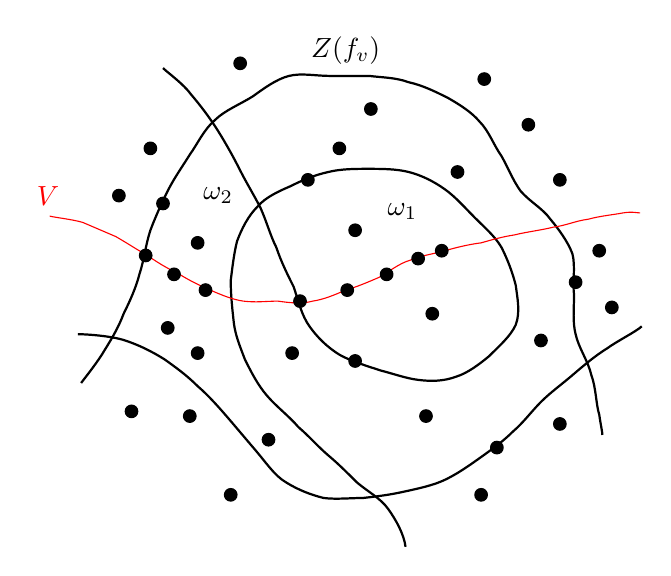
\begin{tikzpicture}[scale=2.0]

  \draw[thick] (0.23,3.61) .. controls (0.26,3.58) and (0.36,3.51) .. (0.41,3.44) .. controls (0.47,3.37) and (0.53,3.29) .. (0.58,3.21) .. controls (0.63,3.13) and (0.68,3.04) .. (0.72,2.96) .. controls (0.76,2.88) and (0.81,2.8) .. (0.85,2.72) .. controls (0.89,2.63) and (0.91,2.55) .. (0.95,2.47) .. controls (0.98,2.38) and (1.02,2.3) .. (1.06,2.22) .. controls (1.09,2.13) and (1.11,2.04) .. (1.16,1.97) .. controls (1.21,1.9) and (1.27,1.84) .. (1.35,1.79) .. controls (1.42,1.75) and (1.52,1.72) .. (1.61,1.69) .. controls (1.69,1.67) and (1.77,1.64) .. (1.85,1.63) .. controls (1.93,1.62) and (2.01,1.62) .. (2.09,1.65) .. controls (2.16,1.67) and (2.24,1.73) .. (2.3,1.78) .. controls (2.36,1.84) and (2.44,1.91) .. (2.47,1.98) .. controls (2.5,2.06) and (2.48,2.15) .. (2.47,2.23) .. controls (2.45,2.31) and (2.42,2.39) .. (2.38,2.47) .. controls (2.34,2.54) and (2.27,2.6) .. (2.21,2.66) .. controls (2.15,2.72) and (2.09,2.79) .. (2.02,2.84) .. controls (1.95,2.89) and (1.87,2.93) .. (1.79,2.95) .. controls (1.71,2.97) and (1.62,2.97) .. (1.53,2.97) .. controls (1.45,2.97) and (1.36,2.97) .. (1.28,2.95) .. controls (1.19,2.93) and (1.12,2.9) .. (1.04,2.86) .. controls (0.97,2.83) and (0.88,2.79) .. (0.83,2.73) .. controls (0.77,2.67) and (0.73,2.59) .. (0.7,2.51) .. controls (0.68,2.43) and (0.67,2.34) .. (0.66,2.26) .. controls (0.66,2.17) and (0.67,2.08) .. (0.68,1.99) .. controls (0.69,1.91) and (0.72,1.84) .. (0.75,1.76) .. controls (0.79,1.68) and (0.83,1.6) .. (0.89,1.53) .. controls (0.95,1.46) and (1.03,1.4) .. (1.09,1.33) .. controls (1.16,1.27) and (1.21,1.21) .. (1.28,1.15) .. controls (1.34,1.1) and (1.4,1.04) .. (1.46,0.98) .. controls (1.53,0.92) and (1.61,0.88) .. (1.66,0.81) .. controls (1.71,0.74) and (1.76,0.65) .. (1.77,0.57) ;



  \draw[thick] (-0.29,1.61) .. controls (-0.26,1.65) and (-0.18,1.75) .. (-0.14,1.82) .. controls (-0.09,1.9) and (-0.05,1.97) .. (-0.02,2.05) .. controls (0.02,2.13) and (0.06,2.22) .. (0.08,2.3) .. controls (0.11,2.39) and (0.12,2.49) .. (0.15,2.58) .. controls (0.18,2.66) and (0.22,2.75) .. (0.26,2.83) .. controls (0.3,2.91) and (0.35,2.98) .. (0.4,3.06) .. controls (0.45,3.13) and (0.49,3.22) .. (0.56,3.28) .. controls (0.62,3.34) and (0.72,3.38) .. (0.8,3.43) .. controls (0.87,3.48) and (0.95,3.54) .. (1.03,3.56) .. controls (1.11,3.58) and (1.2,3.56) .. (1.29,3.56) .. controls (1.37,3.56) and (1.46,3.56) .. (1.54,3.56) .. controls (1.62,3.55) and (1.71,3.55) .. (1.79,3.52) .. controls (1.88,3.5) and (1.96,3.46) .. (2.04,3.42) .. controls (2.11,3.38) and (2.19,3.33) .. (2.24,3.27) .. controls (2.3,3.21) and (2.33,3.12) .. (2.38,3.05) .. controls (2.42,2.98) and (2.45,2.9) .. (2.5,2.83) .. controls (2.56,2.76) and (2.64,2.72) .. (2.69,2.65) .. controls (2.74,2.59) and (2.8,2.51) .. (2.83,2.43) .. controls (2.85,2.35) and (2.83,2.25) .. (2.84,2.17) .. controls (2.84,2.08) and (2.83,2) .. (2.85,1.92) .. controls (2.87,1.83) and (2.93,1.75) .. (2.95,1.66) .. controls (2.98,1.58) and (2.98,1.47) .. (3,1.41) .. controls (3.01,1.34) and (3.02,1.3) .. (3.02,1.28);
  \draw[fill] (2.35,1.2) circle (0.04cm);

  \draw[thick] (-0.31,1.92) .. controls (-0.26,1.92) and (-0.1,1.91) .. (-0.01,1.88) .. controls (0.08,1.85) and (0.16,1.81) .. (0.24,1.76) .. controls (0.31,1.71) and (0.38,1.66) .. (0.45,1.59) .. controls (0.52,1.53) and (0.59,1.45) .. (0.65,1.38) .. controls (0.71,1.31) and (0.76,1.25) .. (0.82,1.18) .. controls (0.88,1.11) and (0.94,1.02) .. (1.01,0.98) .. controls (1.09,0.93) and (1.17,0.9) .. (1.25,0.88) .. controls (1.33,0.87) and (1.42,0.88) .. (1.5,0.88) .. controls (1.59,0.89) and (1.67,0.9) .. (1.76,0.92) .. controls (1.85,0.94) and (1.95,0.96) .. (2.03,1) .. controls (2.11,1.04) and (2.18,1.09) .. (2.25,1.14) .. controls (2.32,1.19) and (2.39,1.24) .. (2.45,1.3) .. controls (2.52,1.36) and (2.57,1.43) .. (2.63,1.49) .. controls (2.69,1.55) and (2.76,1.6) .. (2.83,1.66) .. controls (2.9,1.72) and (2.97,1.78) .. (3.05,1.83) .. controls (3.12,1.88) and (3.24,1.94) .. (3.27,1.97);

  \draw[red] (-0.49,2.67) .. controls (-0.45,2.66) and (-0.35,2.65) .. (-0.28,2.63) .. controls (-0.21,2.6) and (-0.14,2.57) .. (-0.07,2.54) .. controls (0,2.5) and (0.06,2.46) .. (0.13,2.42) .. controls (0.19,2.38) and (0.25,2.34) .. (0.32,2.31) .. controls (0.38,2.27) and (0.46,2.23) .. (0.53,2.2) .. controls (0.6,2.17) and (0.67,2.14) .. (0.74,2.13) .. controls (0.82,2.12) and (0.89,2.13) .. (0.96,2.13) .. controls (1.03,2.12) and (1.11,2.11) .. (1.18,2.13) .. controls (1.25,2.14) and (1.32,2.17) .. (1.39,2.2) .. controls (1.46,2.22) and (1.53,2.25) .. (1.6,2.28) .. controls (1.67,2.32) and (1.73,2.37) .. (1.8,2.39) .. controls (1.87,2.42) and (1.95,2.43) .. (2.02,2.45) .. controls (2.09,2.47) and (2.17,2.49) .. (2.25,2.5) .. controls (2.32,2.52) and (2.39,2.54) .. (2.46,2.55) .. controls (2.54,2.57) and (2.63,2.58) .. (2.71,2.6) .. controls (2.79,2.61) and (2.85,2.64) .. (2.93,2.65) .. controls (3,2.67) and (3.1,2.68) .. (3.15,2.69) .. controls (3.21,2.7) and (3.24,2.69) .. (3.26,2.69);
  \node at (-0.5,2.8) {\color{red} $V$};
  
  \draw[fill] (0.66,0.9) circle (0.04cm);
  \draw[fill] (1.94,2.05) circle (0.04cm);
  \draw[fill] (3.08,2.09) circle (0.04cm);
  \draw[fill] (1.35,3.1) circle (0.04cm);
  \draw[fill] (0.72,3.64) circle (0.04cm);
  \draw[fill] (1.45,2.58) circle (0.04cm);
  \draw[fill] (1.9,1.4) circle (0.04cm);
  \draw[fill] (1.05,1.8) circle (0.04cm);
  \draw[fill] (0.26,1.96) circle (0.04cm);
  \draw[fill] (0.03,1.43) circle (0.04cm);
  \draw[fill] (2.27,3.54) circle (0.04cm);
  \draw[fill] (0.45,2.5) circle (0.04cm);
  \draw[fill] (1.55,3.35) circle (0.04cm);
  \draw[fill] (3,2.45) circle (0.04cm);
  \draw[fill] (2.75,1.35) circle (0.04cm);
  \draw[fill] (0.9,1.25) circle (0.04cm);
  \draw[fill] (0.4,1.4) circle (0.04cm);
  \draw[fill] (2.55,3.25) circle (0.04cm);
  \draw[fill] (2.1,2.95) circle (0.04cm);
  \draw[fill] (2.75,2.9) circle (0.04cm);
  \draw[fill] (-0.05,2.8) circle (0.04cm);
  \draw[fill] (0.15,3.1) circle (0.04cm);
  \draw[fill] (2.25,0.9) circle (0.04cm);
  \draw[fill] (2.85,2.25) circle (0.04cm);
  \draw[fill] (2.63,1.88) circle (0.04cm);

  \draw[fill] (0.12,2.42) circle (0.04cm);
  \draw[fill] (1.1,2.13) circle (0.04cm);
  \draw[fill] (0.23,2.75) circle (0.04cm);

  \draw[fill] (1.45,1.75) circle (0.04cm);

  \draw[fill] (1.15,2.9) circle (0.04cm);

  \draw[fill] (1.4,2.2) circle (0.04cm);

  \draw[fill] (1.65,2.3) circle (0.04cm);

  \draw[fill] (2,2.45) circle (0.04cm);

  \draw[fill] (1.85,2.4) circle (0.04cm);

  \draw[fill] (0.3,2.3) circle (0.04cm);

  \draw[fill] (0.5,2.2) circle (0.04cm);
  \node at (0.58,2.8) {$\omega_2$};
\node at (1.75,2.7) {$\omega_1$};

  \draw[fill] (0.45,1.8) circle (0.04cm);
  \node at (1.39,3.72) {$Z(f_v)$};
\end{tikzpicture}
\end{center}
\caption{An illustration of the space-cutting in dimension 2. Assume $v$ is a vertex of the partition tree at depth $\ell-1$. The union of the black curves is the zero-set of the cutting polynomial $f_v$; $\omega_1,\omega_2$ are two cells, and the red curve is an algebraic surface $V$. The incidences of $V$ with the points of $Q_v\cap Z(f_v)$ are in category 2.  The incidences of $V$ with the points of $Q_v\cap \omega_1$ are in category 3, because the points $\omega_1\cap Q_v \cap V$ span $V$. On the other hand, the incidences of $V$ with the points in $Q_v\cap \omega_2$ are in category 4, because $\omega_2\cap Q_v\cap V $ does not span $V$.}
\label{fig:1}
\end{figure}

		
		We divide the incidences into four categories. Let $(x\in V)$ be an incidence, where $x\in Q$ and $V\in \mathcal{V}$, and let $P$ be an irreducible polynomial such that $V=Z_{\mathbb{R}}(P)$. Then the four categories are
		\begin{enumerate}
			\item $x\in Z_v$ for some inner node $v$ and $P\mid f_v$;
			\item $x\in Z_v$ for some inner node $v$ and $P\nmid f_v$;
			\item $x\in Q_v$ for some leaf node $v$ and $V\cap Q_v$ spans $V$;
			\item $x\in Q_v$ for some leaf node $v$ and $V\cap Q_v$ does not span $V$.
		\end{enumerate}
		See \Cref{fig:1} for an illustration. For $i\in [4]$, let $M_i\in \{0,1\}^{\mathcal{V}\times Q}$ be the matrix recording the incidences in category $i$, that is, $M_i(V,x)=1$ iff $(x\in V)$ is an incidence of category $i$. Then $M=M_1+M_2+M_3+M_4$, and we bound $\gamma_2(M_i)$ for all four matrices individually.
		
		\begin{claim}
			$$\gamma_2(M_1)\leq2 B^{\ell/2}\sqrt{T}.$$
		\end{claim}
		
		\begin{proof}
			Let $v$ be an inner node of the partition tree, and let $N_v$ denote the submatrix of $M_1$, whose columns are indexed by the elements of $Z_v$. If $P\mid f_v$, then $P$ is one of the irreducible components of $f_v$. As the degree of $f_v$ is at most $T$, $f_v$ has at most $T$ irreducible components. This shows that $N_v$ has at most $T$ non-identical non-zero rows, so $\gamma_2(N_v)\leq \sqrt{T}$.
			
			Now for $j=0,\dots,\ell-1$, let $N_{j}$ be the concatenation of the matrices $N_v$ for the internal nodes $v$ on depth $j$. As every $V\in \mathcal{V}$ is active for at most $B^j$ nodes at depth $j$, we can apply \Cref{lemma:concatenation} to $M_j=(N_v)_{v\text{ is at depth }j}$ with parameters $t=B^j$ and $\gamma=\sqrt{T}$ to get
			$$\gamma_2(N_j)\leq B^{j/2}\sqrt{T}.$$
			Finally, as $M_1=(N_0\dots N_{\ell-1})$, we have
			$$\gamma_2(M_1)\leq \sum_{j=0}^{\ell-1}\gamma_2(N_j)\leq 2 B^{\ell/2}\sqrt{T}.$$
		\end{proof}
		
		\begin{claim}
			$$\gamma_2(M_2)\leq \sum_{j=0}^{\ell-1}B^{j/2}f_{D-1,kT}\left(\frac{n}{R^j}\right).$$
		\end{claim}
		\begin{proof}
			Let $v$ be a node of the partition tree, and let $N_v$ denote the submatrix of $M_2$, whose columns are indexed by the elements of $Z_v$. If $x\in Z_v\cap Z_{\mathbb{R}}(P)$, then $x\in Z_{\mathbb{R}}(f_v,P)$. By B\'ezout's theorem, if $P\nmid f_v$, then $Z_{\mathbb{C}}(f_v,P)$ has dimension at most $d-2$ and degree at most $(\deg P)(\deg f_v)\leq kT$. Thus, $N_v$ is an incidence matrix of $Z_v$ with affine algebraic sets of dimension at most $d-2=D-1$ and  degree at most $kT$. Therefore,
			$$\gamma_2(N_v)\leq f_{D-1,Tk}(|Z_v|)\leq f_{D-1,Tk}(|Q_v|).$$
			
			For $j=0,\dots,\ell-1$, let $N_{j}$ be the concatenation of the matrices $N_v$, where $v$ is an internal node of the partition tree at depth $j$. As every $V\in \mathcal{V}$ is active for at most $B^j$ such nodes, we can apply \Cref{lemma:concatenation} to $N_j$ with parameter $t=B^j$ to get
			$$\gamma_2(N_j)\leq B^{j/2}f_{D-1,kT}\left(\frac{n}{R^j}\right).$$
			Here, we used that $|Q_v|\leq n/R^j$ for every node $v$ at depth $j$.
			Finally, as $M_2=(N_0\dots N_{\ell-1})$, we have
			$$\gamma_2(M_2)\leq \sum_{j=0}^{\ell-1}\gamma_2(N_j)\leq \sum_{j=0}^{\ell-1}B^{j/2}f_{D-1,kT}\left(\frac{n}{R^j}\right).$$
		\end{proof}
		
		\begin{claim}
			$$\gamma_2(M_3)\leq O\left(\left(\frac{n}{R^{\ell}}\right)^{L_{d,k}/2-1}\right).$$
		\end{claim}
		\begin{proof}
			Let $v$ be a leaf vertex of the partition tree and let $x_0\in Q_v$. Recall that $|Q_v|\leq n/r=n/R^{\ell}$. Let $\mathcal{V}_{x_0}$ be the set of hypersurfaces $V\in \mathcal{V}$ such that $x_0\in V$ and $V\cap Q_v$ spans $V$. Then by \Cref{lemma:spanning}, there is a set $T_V\subset V\cap Q_v$ of size $L_{d,\deg(V)}-1$ that contains $x_0$ and spans $V$. As $T_V$ uniquely determines $V$, we get that 
			$$|\mathcal{V}_{x_0}|\leq \sum_{i=1}^k \binom{|Q_v|-1}{L_{d,i}-2}=O\left(\left(\frac{n}{r}\right)^{L_{d,k}-2}\right).$$
			This proves that every column of $M_3$ has at most $\left(\left(\frac{n}{r}\right)^{L_{d,k}-2}\right)$ one entries, implying
			$$\gamma_2(M_3)\leq O\left(\left(\frac{n}{r}\right)^{L_{d,k}/2-1}\right).$$
		\end{proof}
		
		\begin{claim}
			$$\gamma_2(M_4)\leq B^{\ell/2}f_{D-1,k^2}\left(\frac{n}{r}\right).$$
		\end{claim}
		
		\begin{proof}
			Let $v$ be a leaf vertex of the partition tree and let $N_v$ be the submatrix of $M_4$, whose columns are indexed by the elements of $Q_v$. Let $V\in \mathcal{V}$ such that $V\cap Q_v$ does not span $V$, and let $P$ be an irreducible polynomial such that $V=Z_{\mathbb{R}}(P)$. Then there exists some $P'\in \mathcal{I}_{\deg(P)}(V\cap Q_v)\setminus \text{span}_{\mathbb{R}}\{P\}$. As $\deg(P')\leq \deg(P)$, we have that $P\nmid P'$. Hence, by B\'ezout's theorem, $Z_{\mathbb{C}}(P,P')$ is an affine algebraic set of dimension at most $d-2$ and degree at most $\deg(P)\deg(P')\leq k^2$. Therefore, $N_v$ is the incidence matrix of $Q_v$ with affine algebraic sets of dimension at most $d-2=D-1$ and degree at most $k^2$, which gives
			$$\gamma_2(N_v)\leq f_{D-1,k^2}(|Q_v|)\leq f_{D-1,k^2}\left(\frac{n}{r}\right).$$
			Finally, $M_4$ is the concatenation of the matrices $N_v$, where $v$ is a leaf node. Each $V\in \mathcal{V}$ is active for at most $B^{\ell}$ leaf nodes, so we can apply \Cref{lemma:concatenation} with parameter $t=B^{\ell}$ to get
			$$\gamma_2(M_4)\leq B^{\ell/2}f_{D-1,k^2}\left(\frac{n}{r}\right).$$
		\end{proof}
		
		Next, we use our induction hypothesis $f_{D-1,k^2}(u)\leq f_{D-1,kT}(u)= O_{D,k,T}(u^{1/2-1/2(d-1)})$, and choose our parameters $T$ and $\ell$, which then define $r,B,R$ as well. Let $\mu=(100L_{d,k})^{-1}$ and $\delta=\mu(100d)^{-2}$. Set
		$$\theta:=\frac{\log B}{\log R}=\frac{(d-1)\log T+\log C_{d,k}}{d\log T+\log c_{d}}=\frac{d-1}{d}+O_{d,k}\left(\frac{1}{\log T}\right),$$
		and choose $T>1$ minimal such that $\theta\leq \frac{d-1}{d}+\delta$. Then $T$ depends only on $d$ and $k$. Choose $\ell$ minimal such that $r=R^{\ell}>n^{1-\mu}$. Then $r=\Theta_{d,k}(n^{1-\mu})$. Rewriting our previous four claims, we have 
		\begin{align*}
			1.\quad \gamma_2(M_1)&\leq 2 B^{\ell/2}\sqrt{T}=2\sqrt{T} R^{\theta \ell/2}\ll_{d,k} n^{(\frac{1}{2}-\frac{\mu}{2})(1-\frac{1}{d}+\delta)}\leq n^{\frac{1}{2}-\frac{1}{2d}-\delta},\\
			2.\quad\gamma_2(M_2)&\leq \sum_{j=0}^{\ell-1}B^{j/2}f_{D-1,kT}\left(\frac{n}{R^j}\right)\ll_{d,k} \sum_{j=0}^{\ell-1} R^{\theta j/2} \left(\frac{n}{R^j}\right)^{\frac{1}{2}-\frac{1}{2(d-1)}}\\
			&\leq \sum_{j=0}^{\ell-1} n^{\frac{1}{2}-\frac{1}{2(d-1)}} R^{\frac{j}{2}(\delta+\frac{1}{d-1}-\frac{1}{d})}\ll n^{\frac{1}{2}-\frac{1}{2(d-1)}} R^{\frac{\ell-1}{2}(\delta+\frac{1}{d-1}-\frac{1}{d})}\\
			&\ll n^{\frac{1}{2}-\frac{1}{2(d-1)}} n^{(\frac{1}{2}-\frac{\mu}{2})(\delta+\frac{1}{d-1}-\frac{1}{d})}=n^{\frac{1}{2}-\frac{1}{2d}+\frac{\delta}{2}-\frac{\mu\delta}{2}-\frac{\mu}{2(d-1)d}}\leq n^{\frac{1}{2}-\frac{1}{2d}-\delta}\\
			3.\quad\gamma_2(M_3)&\ll \left(\frac{n}{R^{\ell}}\right)^{L_{d,k}/2-1}\leq n^{\mu (L_{d,k}/2-1)}\leq n^{1/5}\\
			4.\quad\gamma_2(M_4)&\leq B^{\ell/2}f_{D-1,k^2}\left(\frac{n}{r}\right)\leq n^{\frac{1}{2}-\frac{1}{2d}-\delta}.
		\end{align*}
		Here, the calculations for $\gamma_2(M_4)$ are identical to the calculations for $\gamma_2(M_2)$. Thus, we proved that
		$$g_{d,k}(n)=\gamma_2(M)\leq \sum_{i=1}^{4}\gamma_2(M_i)\ll  n^{\frac{1}{2}-\frac{1}{2d}-\delta}.$$
		It remains to bound $f_{D,k}(n)$ in terms of $g_{d,k}(n)$. Let $Q$ be a set of points in $\mathbb{R}^m$ and let $\mathcal{A}$ be a finite family of affine algebraic sets of dimension at most $D$ and degree at most $k$ such that the incidence matrix $M$ of $Q$ and  $\mathcal{A}$ satisfies $\gamma_2(M)=f_{D,k}(n)$. For $V\in \mathcal{A}$, let
		$$V=X_1\cup\dots\cup X_s$$
		be the decomposition of $V$ into irreducible components over $\mathbb{C}$, then $s\leq k$. Since $V$ is defined over $\mathbb{R}$, complex conjugation permutes the $X_i$'s. In case $X_i\neq \overline{X}_i$, we have
		$$(X_i\cup \overline{X}_i)\cap \mathbb{R}^m=(X_i\cap \overline{X}_i)\cap \mathbb{R}^m$$
		and by B\'ezout's theorem, $\dim(X_i\cap \overline{X}_i)\leq D-1$ and $\deg(X_i\cap \overline{X}_i)\leq k^2$. Let 
		$$V\cap \mathbb{R}^m=Y_1\cup\dots\cup Y_t$$ be the decomposition, where each $Y_i$ is either a component $X_j\cap \mathbb{R}^m$ if $X_j=\overline{X}_j$, or $X_j\cap \overline{X}_j\cap \mathbb{R}^m$ if $X_j\neq \overline{X}_j$. Moreover, in case $t<k$, let $Y_{t+1},\dots,Y_{k}$ be empty sets. For $J\subset [k]$, define the set 
		$$V_J=\bigcap_{i\in J}Y_i,$$
		and let $M_J$ be the incidence matrix of $Q$ and the family $\{V_J: V\in \mathcal{A}\}$. Then the inclusion-exclusion formula gives
		$$M=\sum_{J\subset [k], J\neq \emptyset} (-1)^{|J|+1} M_J.$$
		Here, if $|J|\geq 2$, then $V_J$ is an affine algebraic set of dimension at most $D-1$ and degree at most $k^{2k}$ by repeated applications of B\'ezout's theorem. Thus, 
        $$\gamma_2(M_J)\leq f_{D-1,k^{2k}}(n)\ll_{D,k} n^{\frac{1}{2}-\frac{1}{2D}}\leq  n^{\frac{1}{2}-\frac{1}{2(D+1)}-\delta}.$$ In case $J=\{j\}$ for some $j\in [k]$, we can decompose $M_J$ into $M_{J,1}$ and $M_{J,2}$ along the rows depending on whether $Y_j$ has dimension $D$ or at most $D-1$, respectively. Then $\gamma_2(M_{J,2})\leq f_{D-1,k^2}(n)=O_{D,k}(n^{1/2-1/2D})$ as well. Finally, by the Projection lemma (\Cref{lemma:projection}), there is an affine linear projection $\pi:\mathbb{R}^m\rightarrow\mathbb{R}^{D+1}$ that maps the $D$-dimensional irreducible components $X_i$ (where $X_i=\overline{X}_i$) to irreducible hypersurfaces in $\mathbb{R}^{D+1}=\mathbb{R}^d$ of degree at most $k$ such that for $x\in Q$, we have $x\in Y_i\iff \pi(x)\in \pi(Y_i)$. Therefore, $M_{J,1}$ is the incidence matrix of $\pi(Q)$ and irreducible hypersurfaces in $\mathbb{R}^{d}$ of degree at most $k$, showing $$\gamma_2(M_{J,1})\leq g_{d,k}(n)\leq O_{D,k}\left(n^{\frac{1}{2}-\frac{1}{2(D+1)}-\delta}\right).$$
		In conclusion,
		$$\gamma_2(M)\leq \sum_{J\subset [k], J\neq \emptyset} \gamma_2(M_J)= O_{D,k}\left( n^{\frac{1}{2}-\frac{1}{2(D+1)}-\delta}\right).$$
		By observing that  $\delta\gg \frac{1}{L_{D+1,k} D^{2}}\gg D^{-2}\binom{D+1+k}{k}^{-1}$, this finishes the proof.
	\end{proof}

\end{document}
